\chapter{Performance Analysis}
4124 random images was employed in training, 515 random images was employed in validation and 515 random images was employed in testing process. The performance measuring criterias are 'accuracy', 'precision', 'recall', 'IOU' and 'loss function' for the model's evaluation. 

The checkpoint callback is utilized during training, and the model is trained on a train dataset for 20 epochs while utilizing a different validation dataset  for validation. When the model gets its best IoU score on the validation data, the weights will be saved.

While training the model, the CPU performance is shown in below Figure \ref{performance_cpu}. 
\begin{figure}[htp]
    \centering
    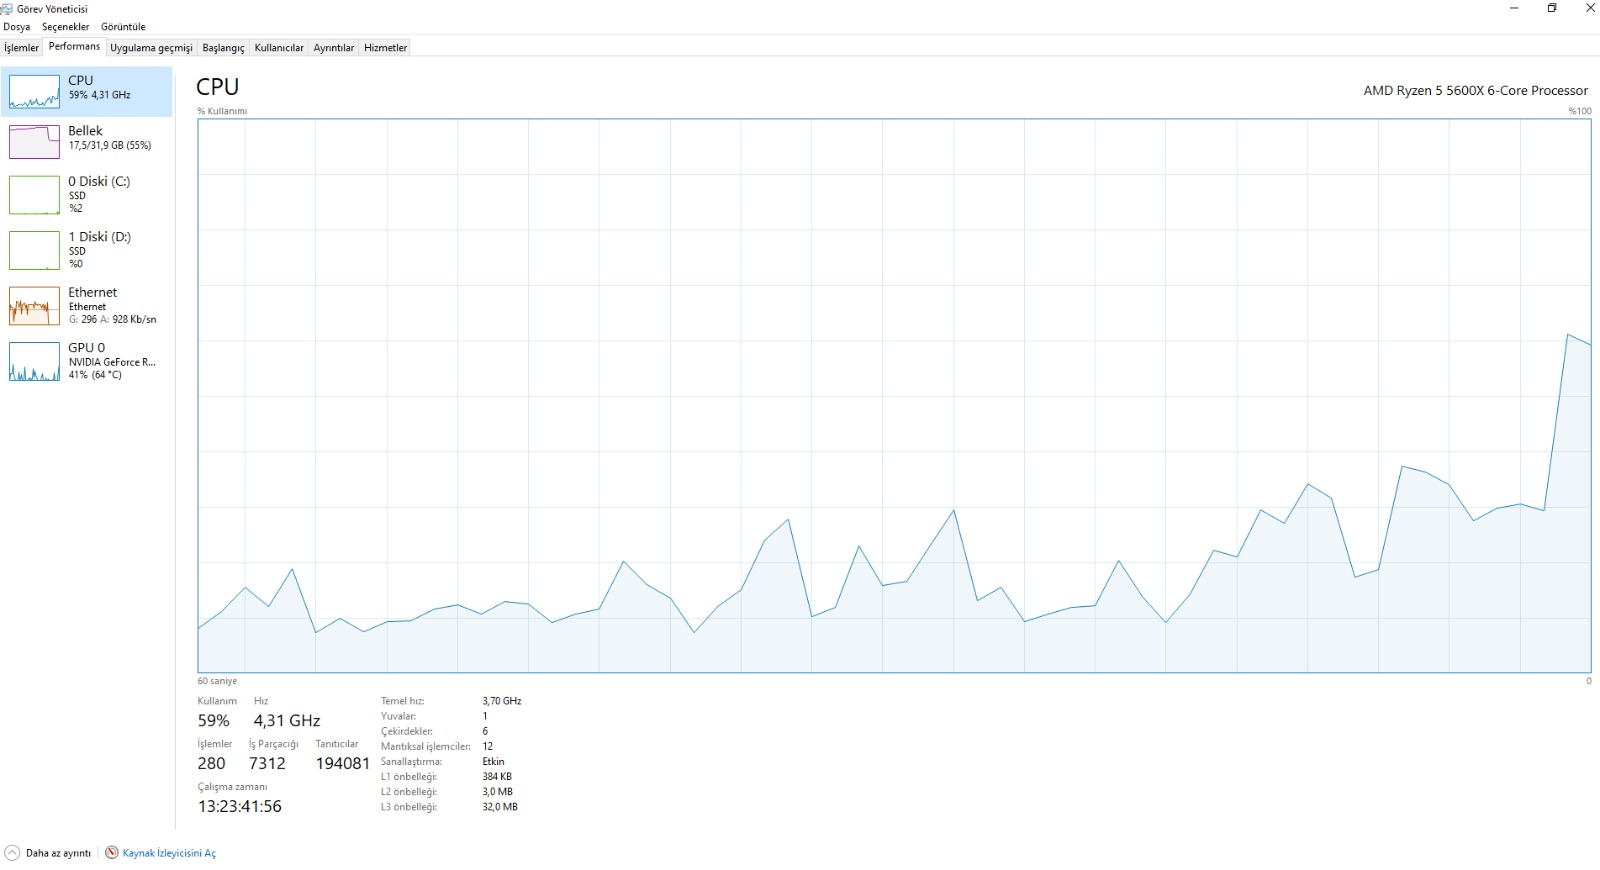
\includegraphics[width=16cm]{projectChapters/images/performance_cpu.jpeg}
    \caption{CPU Usage}
    \label{performance_cpu}
\end{figure}

\newpage
While training the model, the memory performance is shown in below Figure \ref{performance_memory}. 
\begin{figure}[htp]
    \centering
    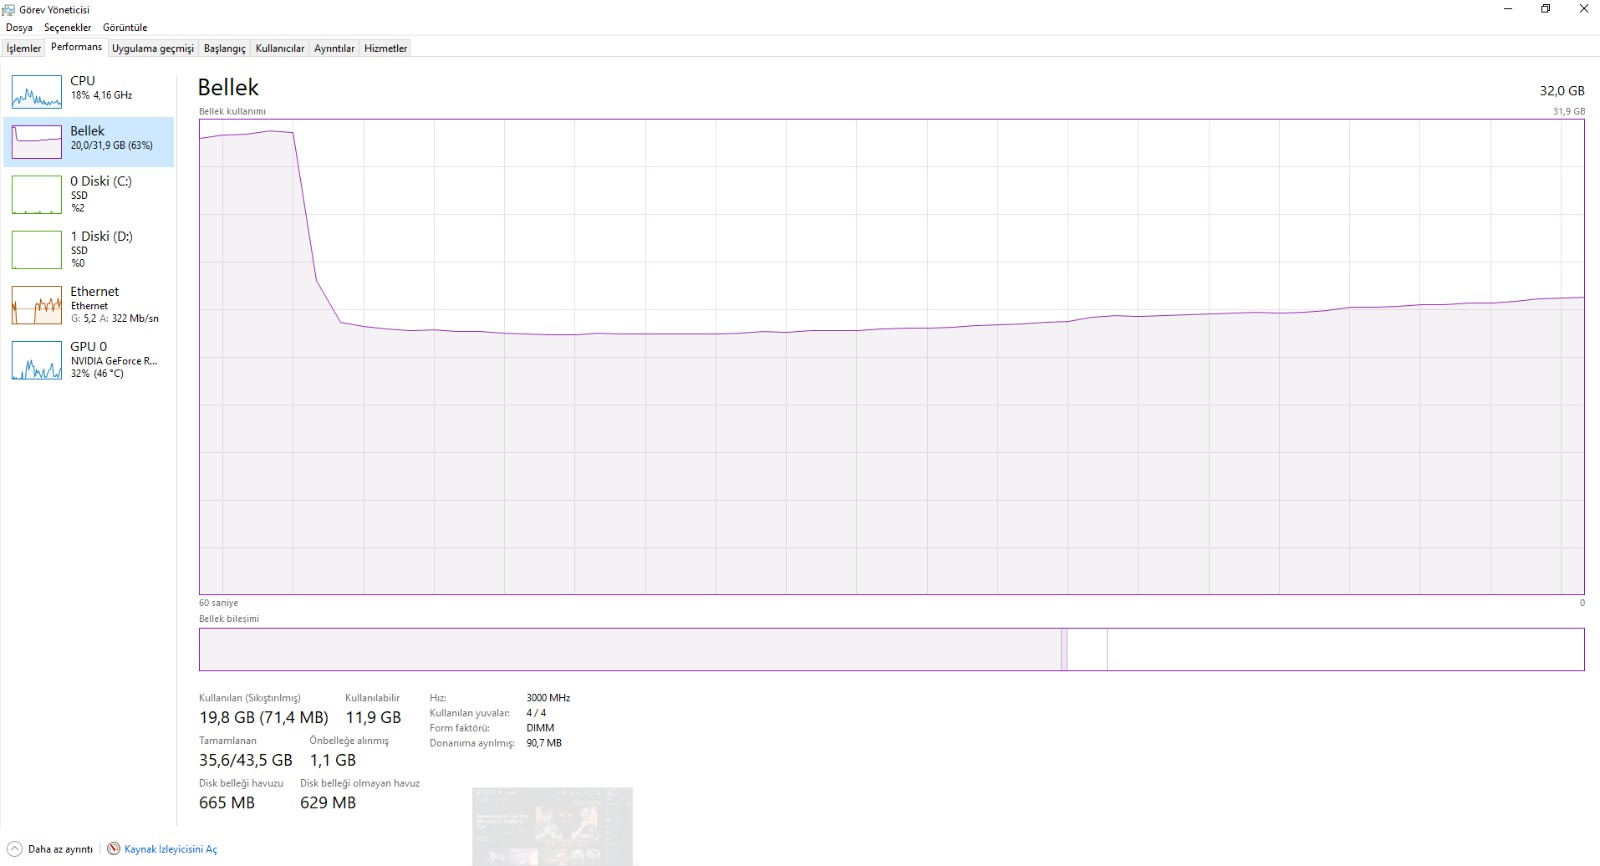
\includegraphics[width=15cm]{projectChapters/images/performance_memory.jpeg}
    \caption{Memory Usage}
    \label{performance_memory}
\end{figure}

While training the model with, the GPU performance is shown in below Figure \ref{performance_gpu}. 
\begin{figure}[htp]
    \centering
    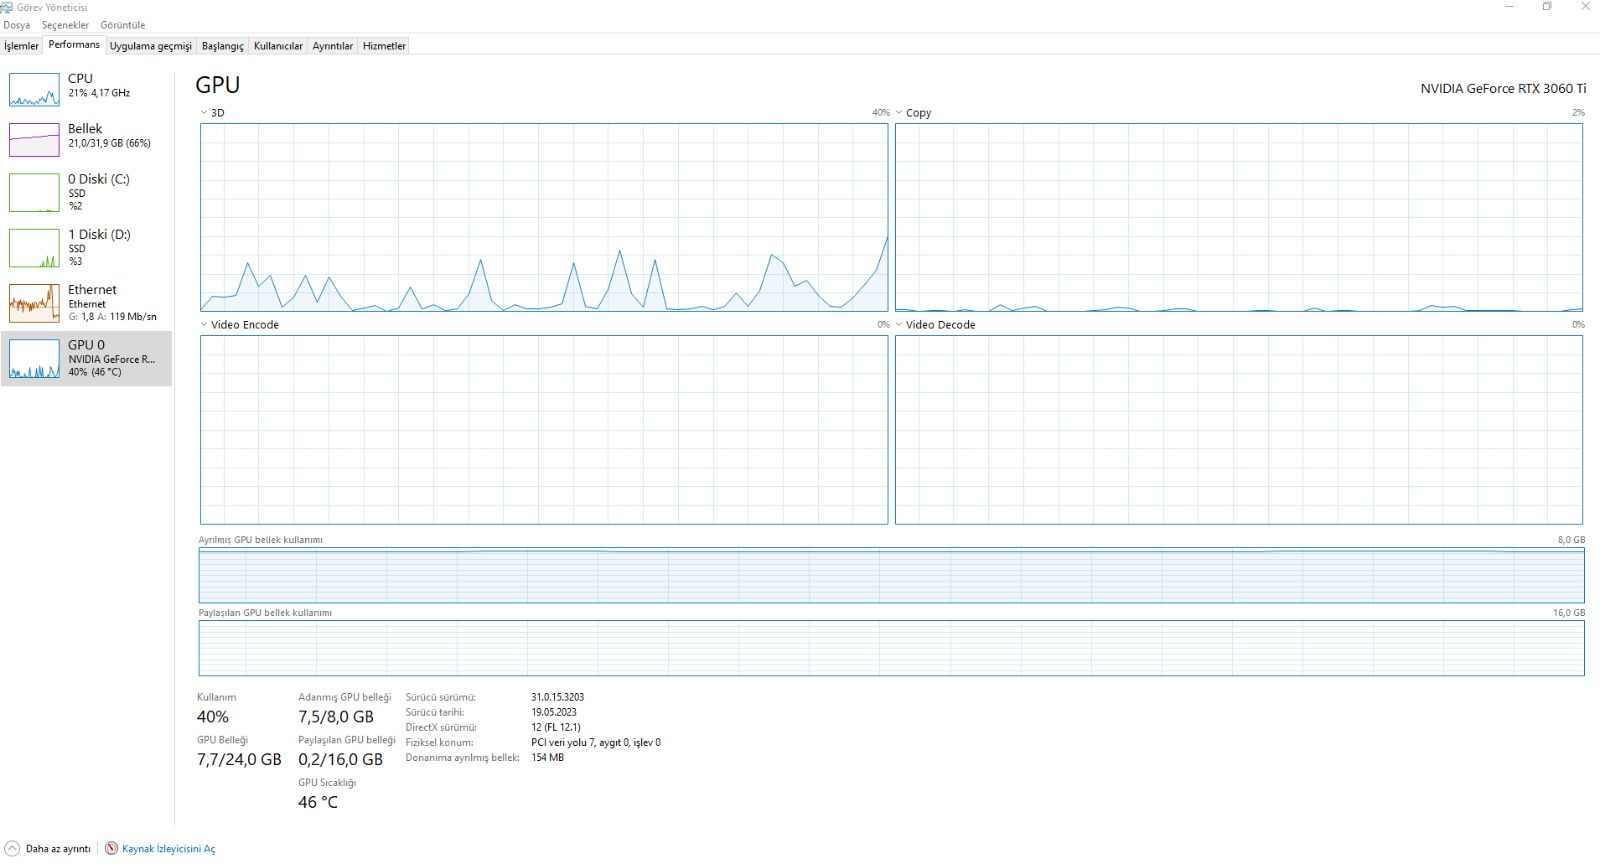
\includegraphics[width=15cm]{projectChapters/images/performance_gpu.jpeg}
    \caption{GPU Usage}
    \label{performance_gpu}
\end{figure}

\newpage
The Figure \ref{epoch_table} below presents the model performance on epochs during training with 4124 train images and 515 validation images. The training had taken 6.91 hours in total. 

\begin{figure}[htp]
    \centering
    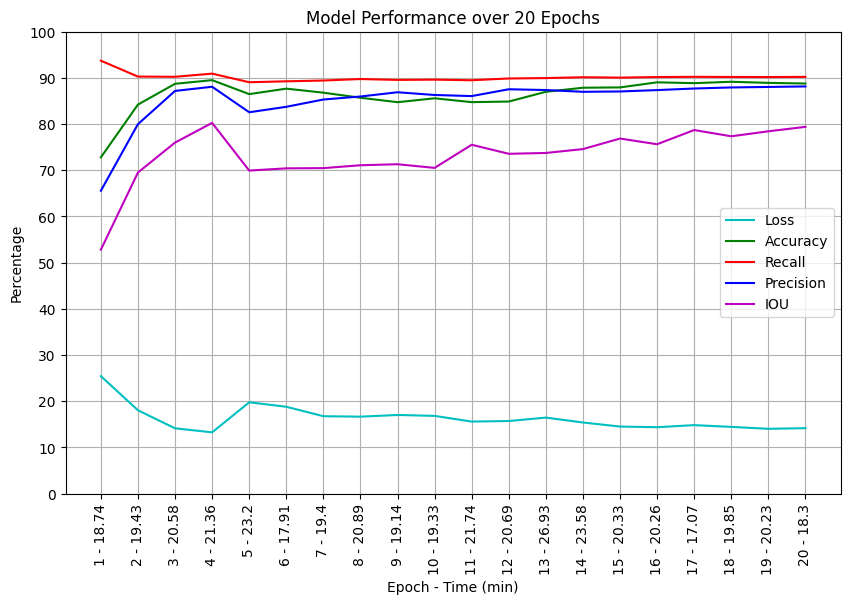
\includegraphics[width=15cm]{projectChapters/images/epoch_table.png}
    \caption{The best weights saved at fourth epoch}
    \label{epoch_table}
\end{figure}
